\section{Evaluation}
\label{eval}

We have used the YFCC100M dataset to evaluate different aspects of our system.
We use the images in the dataset and its associated metadata to implement
an image-search engine based on properties associated with those images.
This is a very common use-case we have encountered when building
applications such as smart-retail, sports applications, and video summarization,
where the starting point is a large set of data that must be curated
before proceeding with the data processing (such as neural network training).
In order to evaluate the different aspects of the performance on the
image search, we have built a baseline following the methodology
used in the industry, and following what we have done in the past
in order to solve the data search problem,
which we describe in Section \ref{images}.

We also evaluate the performance and scalability of the video management
capabilities offered by VDMS.
Handling video in a general way is a complex task.
Some of this complexity comes from the existence of a variety of open and
proprietary implementations, different encoding techniques and container
formats, and different parameters of the video itself that are
application-dependent, like frames per second, lossy compression, etc.
When it comes to video, ad-hoc solutions have a large number of parameters that
can be tuned.
Together with that, there is no system that enables transactional
operations over videos files in the way VDMS does.
Because of this, we focus our efforts on understanding variations in the
performance of VDMS and its scalability, rather than comparing
it to a baseline that would not represent a fair
comparison for either of the systems.
We describe the results in Section \ref{videos}.

Similarly, we explore the behavior of the feature vector functionality in VDMS,
and an evaluation of the different trade-offs that the systems offers for
application developers. For this, we implemented an image-search application
based on \textit{similarity} search, which we describe in Section \ref{features}.


\begin{figure*}
\centering
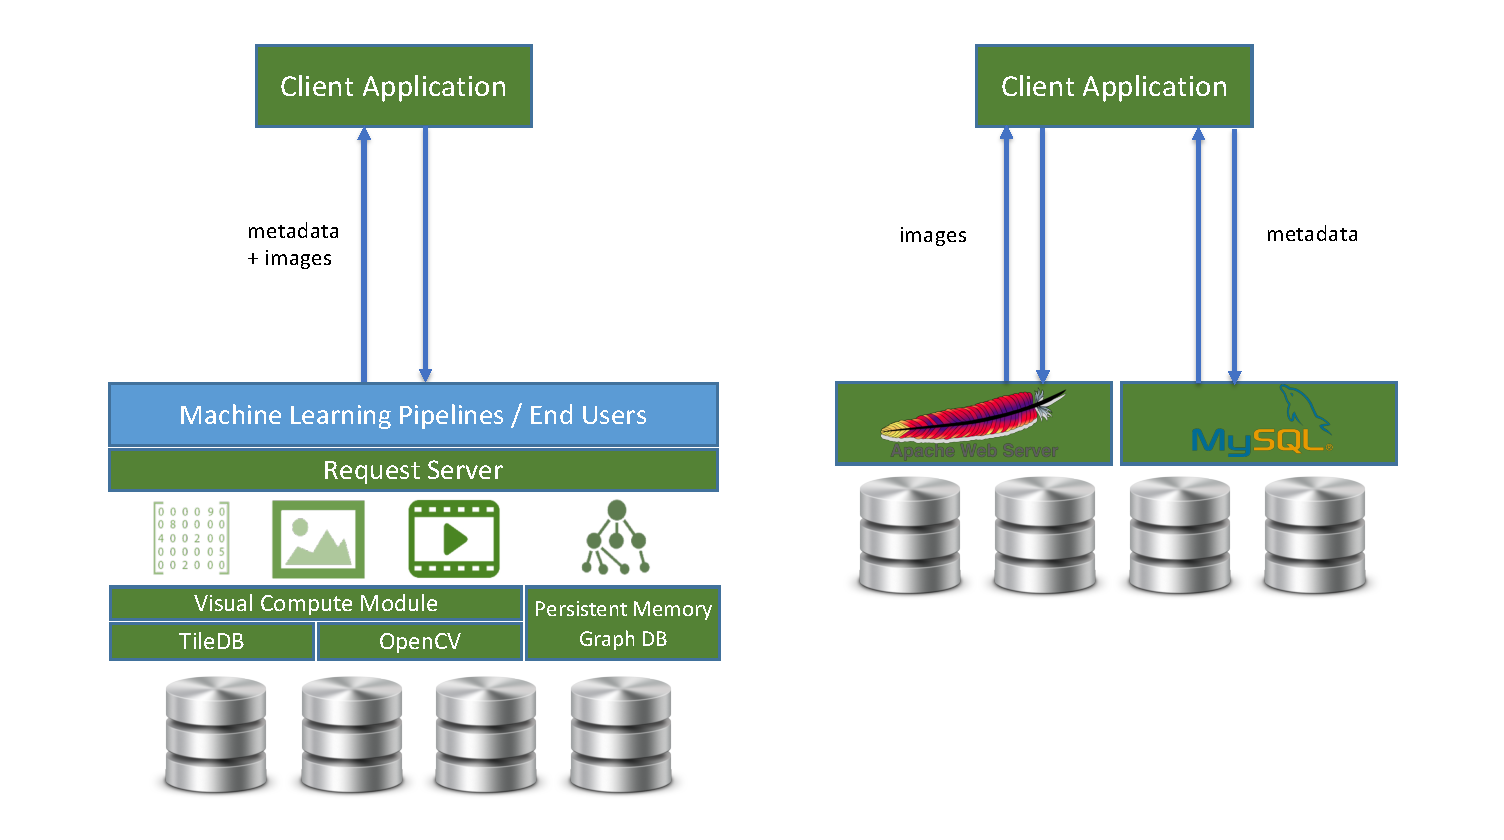
\includegraphics[width=\textwidth]{figures/comparison_system}
\caption{Comparison Systems: Logical view of the interaction between the client application with VDMS (left) and the baseline system (right).}
\label{fig:systems}
\end{figure*}

\subsection{YFCC100M Dataset}
\label{dataset}

The Yahoo! Flickr Creative Commons 100m (YFCC100M) dataset is a large
collection of 100 million public Flickr media objects created to provide free,
sharable multimedia data for research. This dataset contains approximately
99.2 million images and 0.8 million videos with metadata characterized by
25 fields such as the unique identifier, userid,
date the media was taken/uploaded, location in longitude/latitude coordinates,
device type the media was captured, URL to download the media object,
and the Creative Commons license type information.
The YFCC100M dataset also contains \textit{autotags}
provided as a set of comma-separated concepts such as people, scenery, objects,
and animals from 1,570 trained machine learning classifiers ~\cite{Thomee_2016}.
Together with each \textit{autotags}, there is a
probability associated with each tag to indicate certainty of the classification.
This is, an image can have the \textit{autotags} "people", "person", "party",
"outdoor", and each \textit{autotag} assigned will be accompanied by a
probability of that \textit{autotags} being present in that image/frame.
We have also used feature vectors generated for every image and first frame
of every video \cite{features} to implement a similarity search.
Given that there is no standard benchmark oriented towards visual data queries,
we have built a series of queries to filter this dataset that is modeled after
our internal use cases for many of the mentioned applications we have worked
with.

\subsection{Experimental Setup}
\label{setup}

Given that there are no other open-source systems
that implement similar functionality and interfaces as VDMS, as a baseline,
we have implemented an equivalent visual data management system comprised of a
combination of widely available, off-the-shelf components:
MySQL Server 5.7 (for storing metadata),
Apache Web Server 2.4.18 (as interface for image access), and
OpenCV 3.3 (to provide pre-processing operations on images).
Note that this implementation only partially replicates the functionalities
that VDMS offers when it comes to image and metadata handling, built for the
purpose of an ad-hoc image search implementation.
This implementation is based upon internal tools used for
that particular task in the past.
We have implemented a set of client-side applications that take care
of retrieving the components from the different systems, and applies
pre-processing operations when needed.
For visual data workloads, building an approach like the one
implemented as a baseline for this work
is the common practice in the industry \cite{haystack, tao}.

For all our experiments, we use two servers, one hosting a VDMS server and
another hosting the baseline implementation.
Both servers have a dual-socket Intel\textsuperscript{\textregistered}
Xeon\textsuperscript{\textregistered} Platinum 8180 CPU @ 2.50GHz (Skylake),
each CPU with 28 physical cores with hyper-threading enabled,
for a total of 112 logical cores per server.
The server hosting MySQL has 256GB of DDR4 DRAM, while the server hosting VDMS
has 64GB of DDR4 DRAM.
We decided to run VDMS server in the machine with less DRAM to make
sure MySQL had no disadvantage, and because previous evaluation
indicated smaller footprint in the case of VDMS when
compared to similar baselines based on MySQL.
Other than the difference in DRAM space, machines are identical.
Both servers run Ubuntu 16.04.
The client application running the queries and measuring round-trip time
is connected to the server through a 1GB wired link through
a 10GB back-plane switch, same as both servers.

Figure~\ref{fig:systems} shows a logical view of the difference between the
interaction of the client application (retrieves metadata and
images) with VDMS (left) and the baseline (right).
The client application was implemented using Python 3 for both VDMS and
the baseline.

It is worth noting that the images are stored in a shared repository
(ext4 filesystem on a RAID 6 configuration of 16TB) that both 
Apache WebServer and VDMS have direct access. 
In the case of the baseline, metadata is
stored in MySQL using an attached SSD disk.
Even if VDMS has native support for Optane Persistent Memory,
we do not use it in this experiment because of fairness of
comparison with respect to MySQL, which was not designed for
Persistent Memory type of storage.
The benefits of Persistent Memory on metadata operations is left
for another paper, and outside the scope of this evaluation.
For this experiment, in the case of VDMS we simply use a similar
attached SSD disk to store metadata.
Even if PMGD, the graph database used by VDMS, is designed for persistent memory,
it can deliver good performance when using SSDs directly, while still
providing ACID-compliant transactions.

For the metadata, we built VDMS and MySQL databases
using the YFCC100M dataset with incremental database sizes.
For simplicity, we named the database based on the approximate number of images
it contains, as follows: 1M, 5M, 10M, 50M, 100M.
The VDMS and MySQL databases have comparable number of elements. 
The exact number of images/elements in each database are shown in
Table~\ref{table:vdmsnodes} and ~\ref{table:mysqltables}.
The differences can be attributed to failures in data 
preparation/loading because of incomplete/inconsistent formatting, 
which is common in large datasets \cite{failures}.
In our set up, that difference is very small: 
less than 0.1\% in terms of number of elements (images and/or metadata information).

\subsubsection{Data Representation}

\textbf{VDMS:}
For each database size, we created an instance of VDMS using the image/video metadata,
the machine-generated \textit{autotags} associated with
each image/video identifier, and the list of 1,570 \textit{autotags}.
Internally, that information is represented as a property graph,
where we have one node for each image, one node for each tag
(always 1,570 tags), and connections between images.
For instance, if an image has four \textit{autotags} assigned,
there will be four connections between that image and
the different nodes for those \textit{autotags}.
The probability the \textit{autotag} is present in an image
is expressed as a property in the \textit{connection} between the two nodes.
Figure~\ref{fig:graph_representation} shows an example on two images,
two \textit{autotags}, and the \textit{connections} between
those \textit{autotags} and the images.
Image id 23143252 has two \textit{autotags} assigned:
\textit{Alligator} with probability 0.285, and \textit{Lake} with probability 0.872.
Image id 86756231, on the other hand, has a single \textit{autotags} assigned:
\textit{Alligator} with probability 0.894.
On average there are 8 tags assigned to each image so
there will be around 8 times more connections than images, as shown
in Table~\ref{table:vdmsnodes}.
Also, each image node will contain multiple properties associated
with it (some of which are listed in Section \ref{dataset}). 
% Using the Python Client Module, we insert 1,570 nodes for the \textit{autotags},
% and then insert nodes for the YFCC media objects (images or videos)
% with the associated metadata (as properties of the image/video).
% Then, for each image, we add a \textit{connection} between the image node 
% and the \textit{autotag} node. The probability of that \textit{autotag}
% being present in that image is stored as a property in that \textit{connection}.
The number of nodes (representing images and \textit{autotags}) 
are dependent on the database size and the \textit{connections} are responsible for
90\% of the elements in each database instance,  
as shown in Table~\ref{table:vdmsnodes}.

It is important to note that we create indexes for the image identifier,
\textit{autotags} properties, and longitude/latitude coordinates 
to enable faster retrieval.

\begin{figure}[ht]
\centering
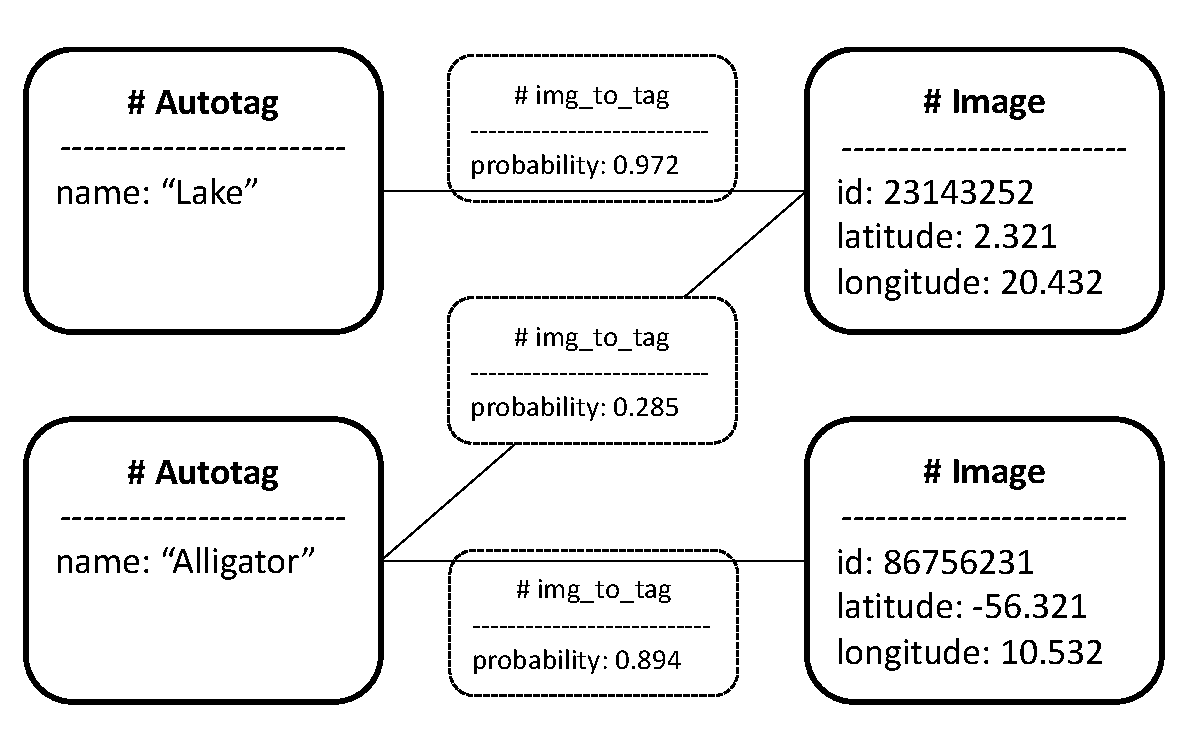
\includegraphics[width=\columnwidth]{figures/graph_representation}
\caption{VDMS Data Representation Using a Property Graph:
Example on two images and 2 \textit{autotags} with
their respective probabilities expressed in the \textit{connection}.
Image id 23143252 has two \textit{autotags} assigned:
\textit{Alligator} with probability 0.285, and \textit{Lake} with probability 0.872.
Similarly, Image id 86756231 has a single \textit{autotags} assigned:
\textit{Alligator} with probability 0.894.}
\label{fig:graph_representation}
\end{figure}

\begin{table}[ht]
\caption{VDMS Database - Number of Elements}
\centering
\begin{tabular}{c c c c}
\hline\hline
DB Name & \# Images & \# Connections & \# TagList\\
\hline
% 100k & 100,000     & 848,432      & 1,570\\
% 500k & 500,000     & 4,249,500    & 1,570\\
1M   & 1,000,000   & 8,503,045    & 1,570\\
5M   & 5,000,000   & 42,505,478   & 1,570\\
10M  & 10,000,000  & 85,040,404   & 1,570\\
50M  & 50,000,000  & 425,162,070  & 1,570\\
100M & 99,205,984  & 895,572,430  & 1,570\\
\hline
\end{tabular}
\label{table:vdmsnodes}
\end{table}

\textbf{MySQL/Baseline:}
Each MySQL database is created in a similar manner as VDMS 
but the data is represented as three tables, following the relational model:
1) \textit{images} table: contains one row per image,
and a column for each property
associated with the images (some of which are listed in Section \ref{dataset});
2) \textit{taglist} table: contains one row per autotag element
(always 1,570 rows);
3) \textit{autotags} table: contains one row per autotag
assigned to an image. Each row contains a foreign key to the
image, a foreign key to the tag, and
the probability assigned to that tag belonging to that image.
Given that there are 8 autotags, on average, per image, the \textit{autotags}
table has around 8 times the number of rows present in the
\textit{metadata} table, as can be seen in Table~\ref{table:mysqltables}.
Using a Python client and simple queries, the \textit{taglist}
table is read from the list of tags with an auto-incremented
\textit{tagid} as a primary key, and the metadata table
is read from the YFCC100M metadata using the identifier as a primary key.
The \textit{autotags} table contains the generated autotags and
probabilities for entries of the \textit{images} table.
To generate the table, we split the \textit{autotags} data for each database
by the image identifier and autotag into new files.
The new files are read into the \textit{autotags} table with the image
identifier and \textit{tagid} as foreign keys.

In an attempt to have the best MySQL configuration possible for this use case, 
we explore several parameters to increase the performance of both loading the data, 
as well as executing the queries.
In particular, MySQL optimizes threads and transactions out-of-box, 
but it cannot handle the entire YFCC100M dataset without configuring 
specific parameters.
When creating large databases, a data lock may occur to protect the
data from concurrent updates~\cite{mysql_blog}.
To avoid this mechanism, we increased the buffer pool size to
increase the amount of memory allocated to internal data structures.
It is recommended to set the buffer pool size to 60-80\% of the physical
memory size ~\cite{mysql,mysql_blog}.
However, the time to build a database increased. 
We later changed  the buffer pool size to a multiple of the default value, i.e. 16x,
which produced the best results for loading time.

By default, MySQL uses the available operating system threads to  
execute \textit{n} requests in parallel where \textit{n} is 
the number of background read/write I/O threads.
Setting the respective parameters in the MySQL configuration file can limit the
number of concurrent threads and the number of background threads.
When a limit is set on the number of threads, and no threads are available,
requests will go into a FIFO queue until threads are available to execute
the request ~\cite{mysql,mysql_blog}.
We ran a few experiments investigating the effects of setting a limitation on the
number of concurrent and background threads.
We concluded that the default settings perform better for large databases instead of
setting a limit.
Therefore, we let MySQL to automatically handle the concurrency.

In the case of VDMS, we did not attempt to tune any
parameter to avoid unfairness in the comparison against the baseline.
We use the default parameters provided by the implementation.
For both VDMS and the baseline, we created indexes over the 
properties we used for search, such as name of 
\textit{autotag}, and geo-location values.
Building indexes for the right properties and objects
is basic operation that would be present in any real-world deployment,
and measuring performance without them would lead to useless analysis in our
real-world applications and use cases.

\begin{table}[ht]
\caption{MySQL Database - Number of Rows in each Table}
\centering
\begin{tabular}{c c c c}
\hline\hline
 & \multicolumn{3}{c}{Table}\\
\cline{2-4}
DB Name & images & autotags & taglist\\
\hline
% 100k & 100,000    & 848,912     & 1,570\\
% 500k & 498,707    & 4,241,200   & 1,570\\
1M   & 1,000,000  & 8,508,380   & 1,570\\
5M   & 4,987,379  & 42,425,905  & 1,570\\
10M  & 10,000,000 & 85,095,265  & 1,570\\
50M  & 50,000,000 & 425,446,208 & 1,570\\
100M & 99,206,564 & 896,002,496 & 1,570\\
\hline
\end{tabular}
\label{table:mysqltables}
\end{table}

\begin{figure}
\centering
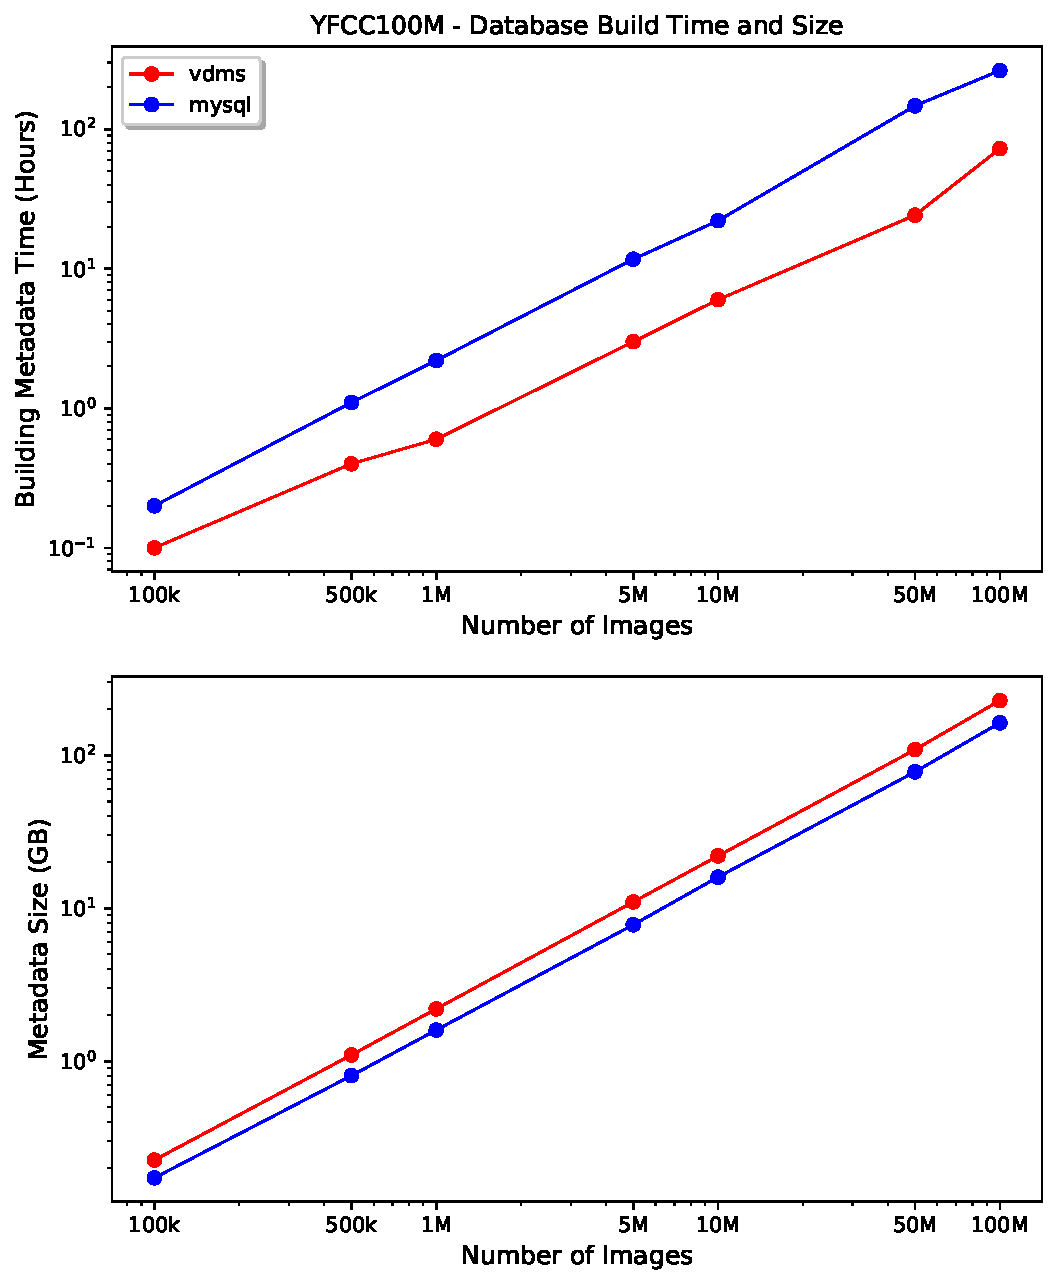
\includegraphics[width=\columnwidth]{figures/db_time_size}
\caption{Time to build and size (in GB) of MySQL and VDMS databases.}
\label{fig:db_time_size}
\end{figure}

\subsubsection{Database Loading Time}

One of the first things we noticed is the difference in loading times,
where VDMS outperforms MySQL by a large margin.
This analysis includes the metadata, as the images are stored in a shared filesystem. 
Figure~\ref{fig:db_time_size} illustrates how VDMS can build databases
faster than MySQL, and how the speedup is sustained as the database size grows.
Key difference in the build times are attributed to the low-level
implementation of how MySQL reads and stores data from the files and the
optimizations (increased InnoDB pool size, etc.) needed
to handle large datasets such as YFCC100M.
On average, it took MySQL around 3.72x longer to build each database than VDMS.

\subsubsection{Database Storage Footprint}

Another important aspect to note is that
VDMS requires more storage for metadata, shown in Figure~\ref{fig:db_time_size}.
This is space used to store information about each node/connection.
The Graph Database internal to VDMS (called PMGD) was designed for performance,
especially in environments where persistent memory is present.
This design decision comes as a trade-off for storage footprint, which is
noticeable in our results.
VDMS required 30-41\% more storage than MySQL for storing the same amount
of metadata.
This may become a factor if storage is a limitation, but it should also be noted
that even if we have a 41\% increase in metadata size,
metadata accounts for less than 2\% of the overall database size.
For example, the largest database (both metadata and images) we built
(100M) has around 230GB of metadata and 12TB of images.
In systems where persistent memory is a scarce resource,
the increased storage foot print of PMGD may represent a challenge.
On the other hand, persistent memory is expected to be available 
in the order of TBs per server, which should fit the 
metadata of intensive use-cases\cite{IntelXPoint15}.

%=========================================

\subsection{Images Search}
\label{images}

In order to evaluate VDMS and the baseline on our use-case queries,
we implemented 4 queries that filter and retrieve a specific set of images.
We chose these queries because they represent typical use-cases where a
cohort of images is to be retrieved and processed from a large corpus of data.
As we mentioned before, we took this approach due to the lack of standard
benchmarks that are oriented towards visual data retrieval.
We use the metadata associated with the images to filter said images.

We use the \textit{autotags} (as they contain information about the content 
of the image), and geo-location information (latitude/longitude) 
of the images for search and filtering.
Note that, even if we use geo-location for our study, any other property 
assigned to the images can be used to refine the search 
in both VDMS and baseline implementations.
On top of that, and for our use cases, we would like to extract more information
about the content of the image through the use of ML,
such as Convolutional Neural Networks~\cite{cnn}.
For this, we resize the images to 224x224, which is the input layer size for
popular variations of neural networks for object detection on images~\cite{resnet}.

To evaluate the access to metadata and images,
we use the following four queries, modeled after our internal use cases:
\begin{itemize}
\item \textit{q1} - {\bf {\em 1tag}}: Find metadata/images with one specific autotag (i.e. alligator, lake, etc).
\item \textit{q2} - {\bf {\em 1tag\_resize}}: Find metadata/images with one specific autotag and resize to 224x224.
\item \textit{q3} - {\bf {\em 1tag\_resize\_geo}}: Find metadata/images with one specific autotag, resize to 224x224, and in a particular geo-location (with a 20 degrees radius in latitude and longitude).
\item \textit{q4} - {\bf {\em 2tag\_resize\_geo}}: Find metadata/images with two specific autotags (i.e. alligator AND lake), resize to 224x224, and in a particular geo-location (with a 20 degrees radius in latitude and longitude).
\end{itemize}

It is important to note that when querying for images with certain
\textit{autotags}, we also apply a filter using the probability.
For instance, we only retrieve images with an autotag \textit{alligator}
and a probability higher than 92\%.
These probabilities are both present in VDMS (in the form of a property
of the \textit{connection} between the image and that \textit{autotag}),
as well as in MySQL (in the form of a column in the \textit{autotags} table
that links images with tags).
In the case of VDMS, the query involves a graph traversal query that starts
from the \textit{autotag} node and ends in the images node,
following \textit{connections} between the image and that \textit{autotag}).
In the case of the baseline implementation,
the query involves JOIN operations between the 3 tables.
The implementation of this evaluation, as well as all the queries, are available
under the benchmarks branch of the VDMS project
\footnote{https://github.com/IntelLabs/vdms/ under benchmark/benckmarks/visual\_storm/yfcc100m},
and some examples of the queries can be found in the appendix of this
paper.

\begin{figure}[ht]
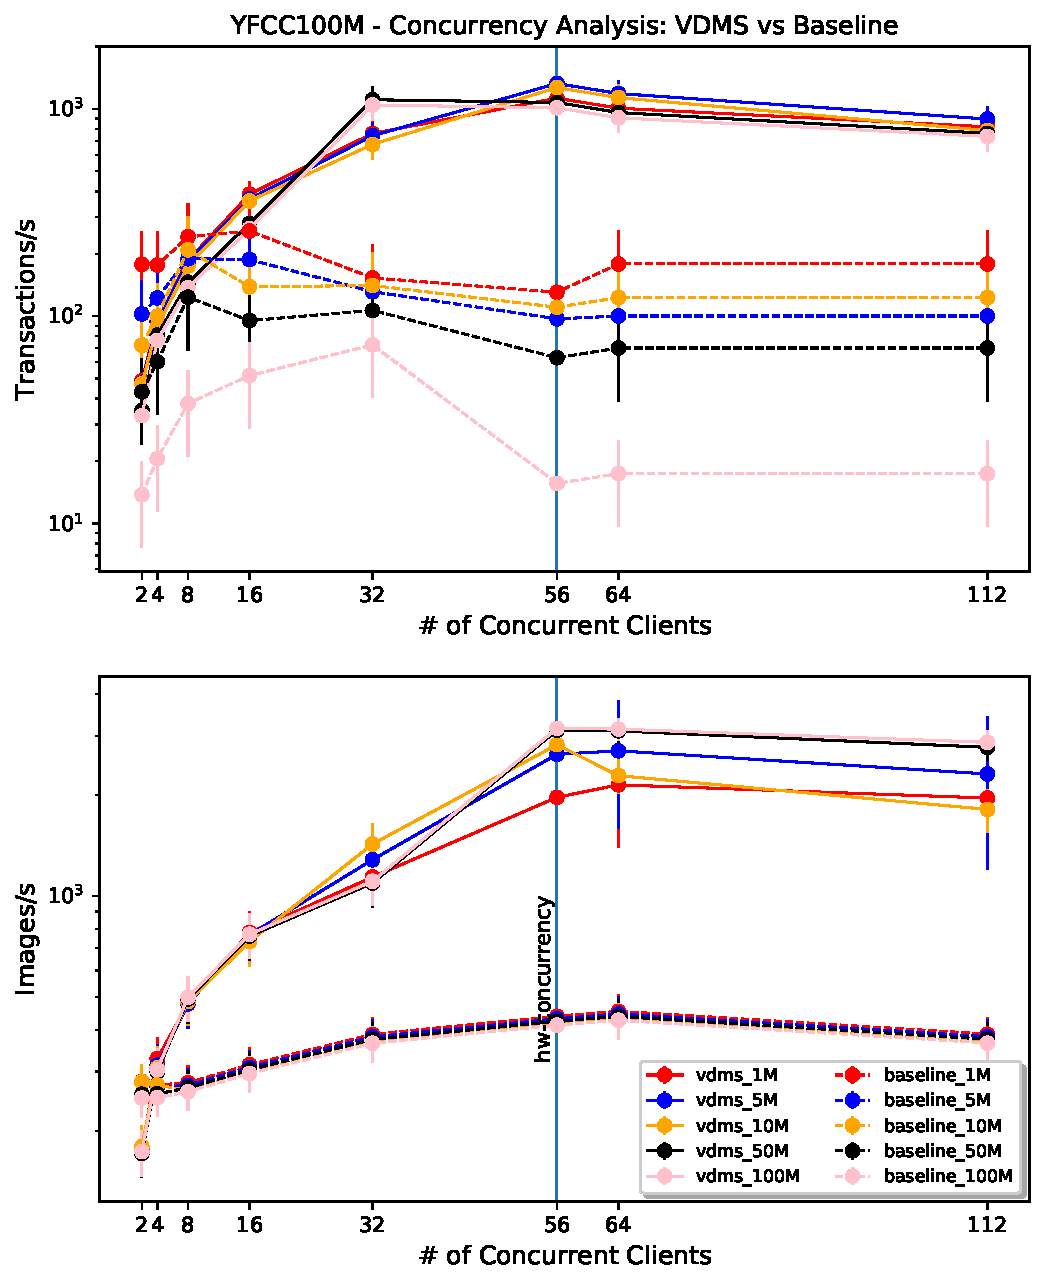
\includegraphics[width=\columnwidth]{figures/concurrency_comparison}
\caption{Concurrency Analysis on \textit{q2} (\textit{1tag\_resize}).
Hardware concurrency (number of physical cores in each system)
is shown with a blue vertical line (hw-concurrency = 56).
Top figure shows aggregated throughput (transactions per second)
when retrieving only metadata associated with the images, as the number of
concurrent clients increase.
Bottom figure shows aggregated throughput (images per second) when retrieving
resized versions of the images, as the number of concurrent clients increases.}
\label{fig:concurrency_comparison}
\end{figure}

Also, note that the size of the result (number of images retrieved)
is linear with the size of the database. This is, if a query returns 100 images
for the 1M database, it will return around 1000 images for the 10M database.
This poses a problem when evaluating performance as the size of the database increase,
and clearly understanding the measurements.
Because of this reason, we control the number of returned images for all the
databases using the probability of the \textit{autotags} 
(higher probabilities returns less images), so that the queries in 
this experiment return a similar number of images for all database sizes.
In other words, as the size of the database increase, we increase the probability
threshold for the queries. We do this for both VDMS and the baseline, of course.
This way, we remove bottleneck introduced by network bandwidth that would
otherwise over-complicate the understanding of the results.

\begin{figure*}[ht!]
\begin{subfigure}{.5\linewidth}
  \centering
  % include first image
  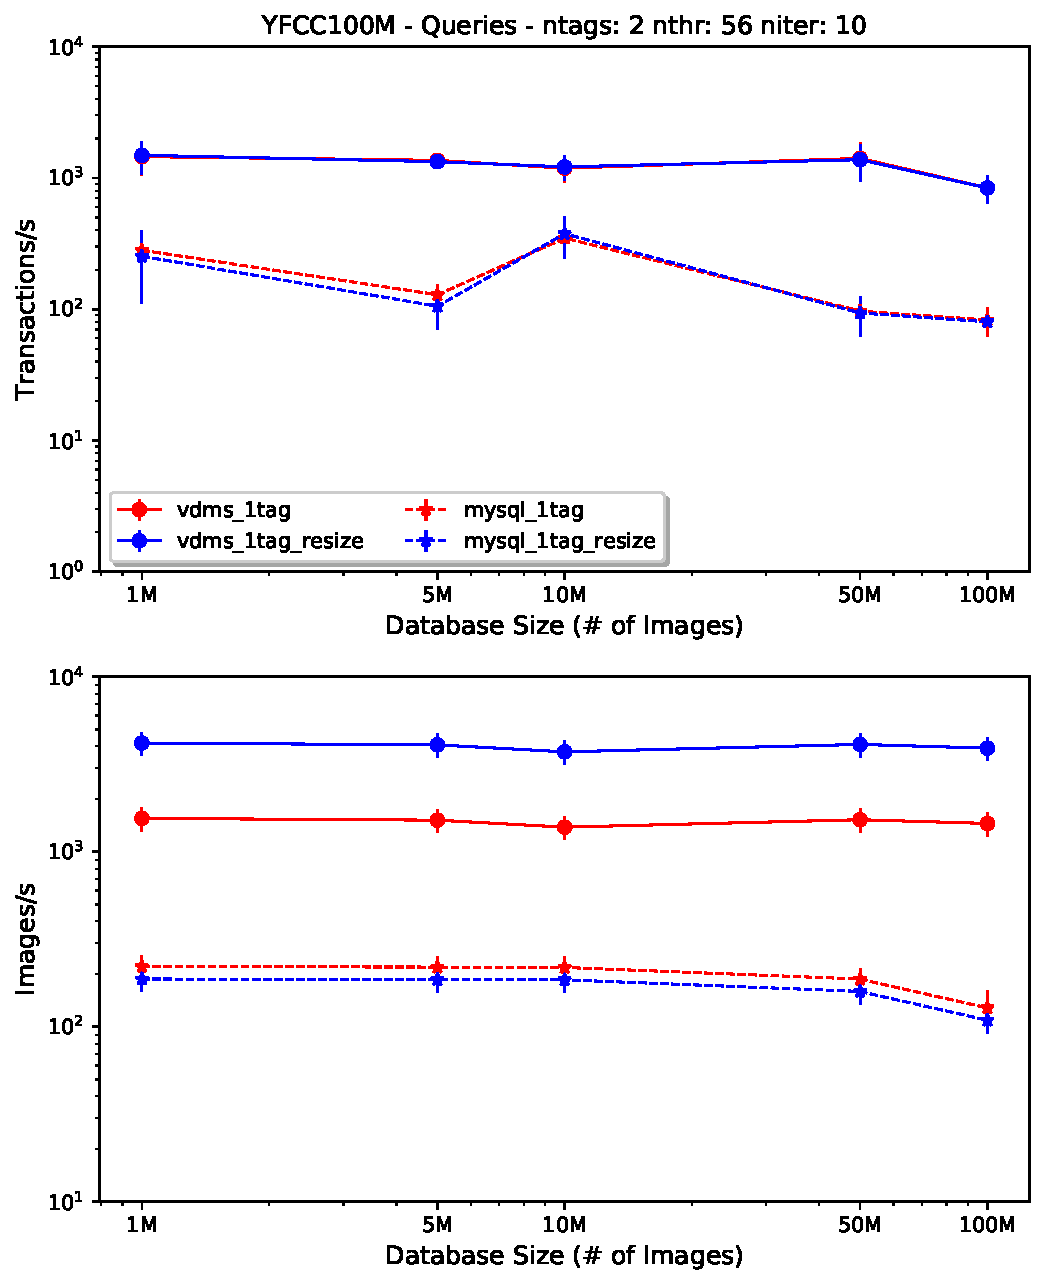
\includegraphics[width=\columnwidth]{figures/queries_throughput_56_q1_q2}
  \caption{\textit{q1}(red), and \textit{q2}(blue).}
  \label{fig:q1_q2}
\end{subfigure}
\begin{subfigure}{.5\linewidth}
  \centering
  % include second image
  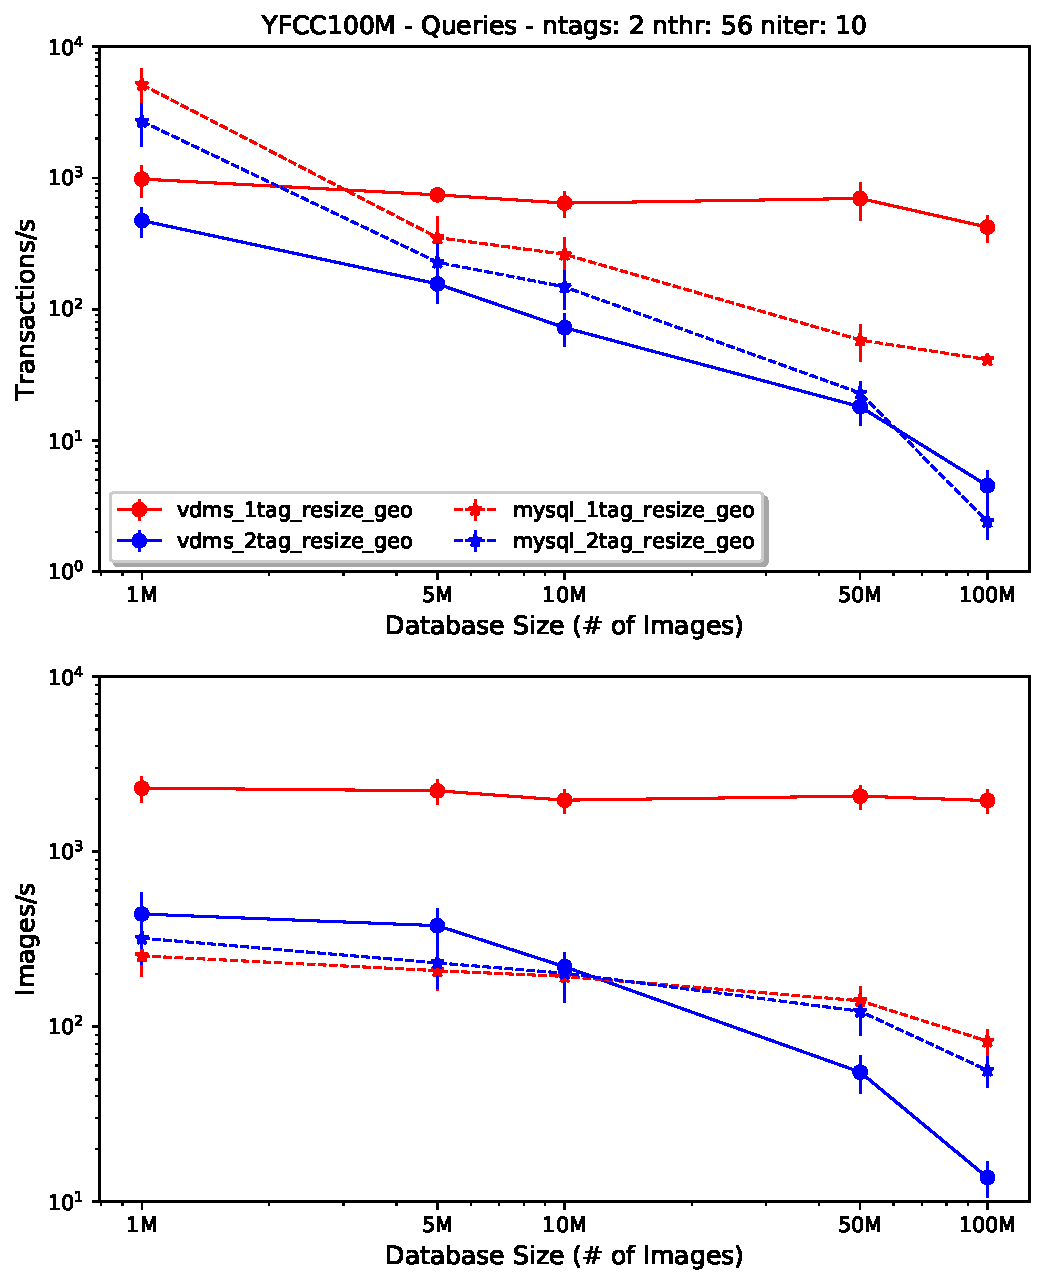
\includegraphics[width=\columnwidth]{figures/queries_throughput_56_q3_q4}
  \caption{\textit{q3}(orange), and \textit{q4}(black).}
  \label{fig:q3_q4}
\end{subfigure}
\caption{Performance Analysis using 4 queries from our use-case
described in the Experimental Setup Section.
We show 2 queries in each figure for readability reasons.
Top figures show the throughput of the 4 queries,
just retrieving metadata associated with the images.
Bottom figures show the throughput when retrieving both metadata and images,
plus operations applied to images when applicable (queries 2, 3 and 4).
The experiments show the performance of both systems (VDMS and baseline) as the
database size increases.
These queries were run using 56 simultaneous clients (nthr = 56),
and averaged out of 10 runs (niter = 10),
each client running 2 transactions (ntags = 2).}
\label{fig:q_throughput_56}
\end{figure*}

Image search based on metadata is very expensive in large databases.
Because of the large volume of data, the processing of the retrieved images
is performed in parallel, using multi-core and/or distributed systems.
For instance, a common implementation of an image processing pipeline
would involve the use of distributed processing frameworks
like Hadoop \cite{hadoop} or Spark \cite{spark}.
Consequently, it is key that the data management system used supports
concurrency, providing multiple workers with data in parallel.
The ability to scale with the number of simultaneous clients is key for the
applicability of visual data management systems like VDMS.
Because of this, we put emphasis on the analysis of concurrency and throughput,
rather than latency.

%% ========= Concurrency Comparison Analysis

\subsubsection{Concurrency Analysis}

Figure~\ref{fig:concurrency_comparison} illustrates a concurrency analysis for
\textit{q2}(\textit{1tag\_resize}), described above,
using both VDMS and the baseline.
Here we evaluate the scalability of both systems, as the number of concurrent
clients grows (x-axis) and as the
size of the databases grows (each full-line represents a database size
for VDMS and each dotted-line represents a database size for the baseline).

We start by analyzing Figure~\ref{fig:concurrency_comparison} (top),
which shows aggregated throughput (transactions per second)
when retrieving only metadata associated with the images, as the number of
concurrent clients increase.
The first thing to notice is that at low concurrency (2 to 8 concurrent clients),
both systems show similar performance, except in the 100M case of the baseline.
Note that, for this particular experiment,
baseline translates directly to MySQL performance,
as the metadata-only queries only involve running a query to MySQL.

For the baseline system, in the case of 100M, the increase in the
size of data seems to have a larger impact in performance.
This result can be attributed to the increase in the complexity of the JOIN
operation as the number of rows in the tables increases.

Another thing to notice is that, as the number of concurrent clients increases,
VDMS throughput continues to increase up to 56 threads, which is
the hardware concurrency of the system.
Also, more parallelism after 56 threads does not increase the delivered throughput,
and it is actually slightly detrimental (112 concurrent clients case).
On the other hand, the baseline seems to deliver less aggregated
throughput after 16 threads, with an increase for 64 threads, but these effects
are hard to interpret fully as the standard deviation in the measurements is high.
We noticed throughout many experiments that MySQL results showed higher
standard deviation, meaning less consistent and noise measurements, when compared
to VDMS.
We tried increasing the number of measurements and discarding
outliers but were not able to get less noisy results.

We continue by looking at Figure~\ref{fig:concurrency_comparison} (bottom),
which shows aggregated images per second delivered by each system.
Again, we evaluate the scalability of both systems, as the number of
concurrent clients grows (x-axis) and as the
size of the databases grows (each full-line represents a database size
for VDMS and each dotted-line represents a database size for the baseline).
Note that most of the baseline dotted-lines are very close to each other.
This is mostly an effect of the log-scale used, which is needed to clearly
depict the difference between VDMS and the baseline.
Here, the baseline is the full architecture described in
Figure~\ref{fig:systems} (right).
Figure~\ref{fig:concurrency_comparison} (bottom) shows a similar trend as the top
figure when it comes to low concurrency. The baseline does as good and even better than VDMS with 2 or 4 concurrent clients.
However, as concurrency increases beyond 4 concurrent clients, the difference
in throughput becomes clear, with VDMS reaching its peak performance at
56 concurrent clients.
This query (as well as \textit{q3} and 4) runs a resize operation on the image,
an operation that requires decoding, resizing, and encoding the image
before sending it back to the client.
These operations are mainly compute bound, and that is the reason for
the system to stop scaling beyond the number of physical cores.
In contrast, the baseline does not scale nearly as well as VDMS,
and we see that even after increasing concurrency, the increase
in throughput is just about 2x.
When comparing the case of 56 or 64 concurrent clients,
VDMS delivers between 8x and 10X the throughput.

There are many reasons why we see this performance improvement, the main being
that the entire operation (metadata query, image fetching and resizing) happens
on the server side in the case of VDMS, within a single message
exchange between the client and the server.
Many of the inefficiencies that come with combining tools that were designed
for other use cases simply disappear when building a tool that treats
visual entities as first class citizens, as it is the case of VDMS.
Another reason, which is quantifiable in the bottom figures, is that
VDMS sends resized (smaller) versions to the client instead of the full image
to be resized on the client side (as is the case in the baseline).
This is in contrast with the baseline, where 2 rounds of blocking back-and-forth
communication with the server is needed, as depicted in Figure~\ref{fig:systems}.
Note that on the point 1), one could argue that the opposite will happen
when the resize operation retrieves a up-sampled (larger) version of the image
instead of a down-sampled (smaller) one.
In practice, retrieving an up-sampled version is not a common use case,
given that up-sampling the image does not add any extra information that can help,
for instance, improve the accuracy of a ML model.
The case of down-sampling the original image is much more common and is the common
practice when it comes to image processing through CNNs \cite{cnn,resnet}.

%% ========= Concurrency Comparison Analysis - END


%% ========= Queries Analysis

\subsubsection{Query Execution Analysis}

The next step in our analysis involved running a different set of queries
(described above in this section),
to better understand the performance of the systems under different query conditions.
Figure~\ref{fig:q_throughput_56} shows the evaluation of the 4 representative
queries we analysed for our use case.
Top figures show the throughput of the 4 queries
retrieving metadata associated with the images.
Bottom figures show the throughput when retrieving both metadata and images,
plus operations applied to images when applicable  (queries 2, 3 and 4).
The experiments show the performance of both systems (VDMS and baseline) as the
database size increases in terms of number of images.
These queries were run using 56 simultaneous clients (nthr = 56),
and averaged over 10 runs (niter = 10),
each client running the retrieval of the tag 2 times (ntags = 2).
The last parameter (ntags) is to avoid having some queries to finish the work
too fast before other clients can even send the query to the server.
This ensures that there is enough work to do in a query so that
all queries execute in parallel on the server side.
To analyze these plots, one needs to compare the full-line (VDMS) versus the
dotted-line (baseline), each color representing a different query.
For example, to compare \textit{q1} performance, one needs to look at
the full-red line (VDMS) and the dotted-red line (baseline).

\begin{figure*}[ht!]
\centering
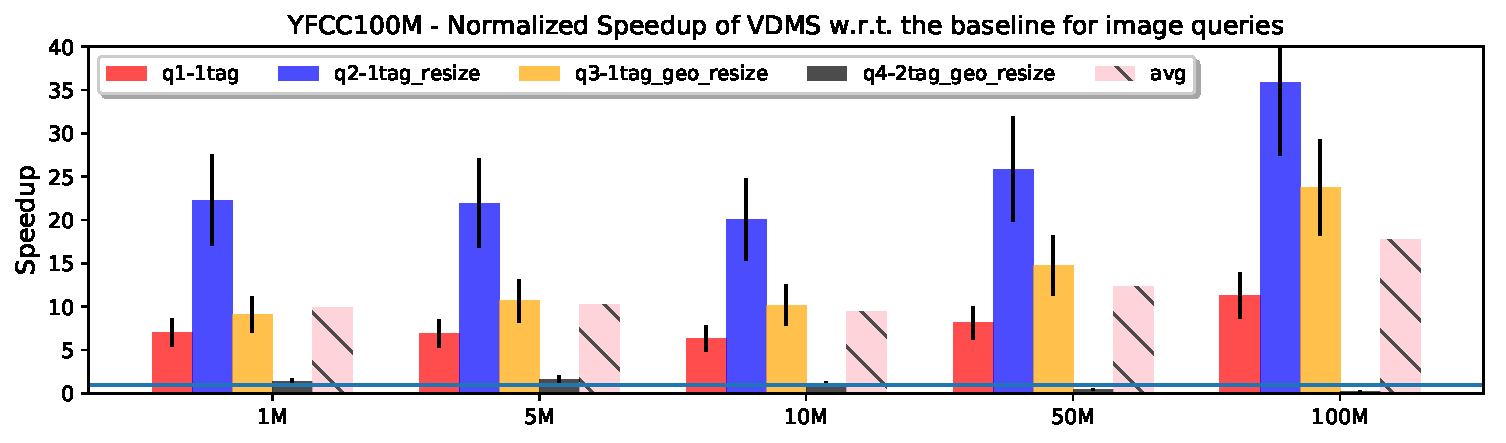
\includegraphics[width=\textwidth]{figures/summary_images}
\caption{Summary of performance gains for all queries.
We see up to 35x speedup (\textit{q2}), and an average of about 15x.
More importantly, we see that the speedup grow as the database size increases,
showing that VDMS scales better than the baseline.}
\label{fig:summary_images}
\end{figure*}

\subsubsection{Metadata Retrieval}

First, we analyze the top figures, showing metadata transactions per second.
We evaluate the performance when retrieving only metadata associated with the images,
and not the images themselves.
In this particular case, the baseline translates directly into MySQL performance.
Note that for these figures (top), \textit{q1} and \textit{q2} are
essentially the same query. This is because the metadata retrieved for both
queries does not change. The only difference between \textit{q1} and \textit{q2}
is the presence of the resize operations that does not have any impact on
analyzing performance of metadata retrieval.
For \textit{q1} and \textit{q2}, we can appreciate higher performance being delivered by
VDMS when compared to the baseline, and how this improvement is maintained
as the size of the database increase.
For \textit{q3}, we see that MySQL performs best when the database size
is small (1M images), with VDMS outperforming MySQL as the database increases in size.
For \textit{q4}, we see MySQL also outperforming VDMS on small size databases, and as
the database size increase, the gap between the two narrows.
It is interesting to note that adding filtering by geo-location
(\textit{q3} and \textit{q4}) slightly increases the performance of MySQL
for small databases, and decreases it as the database sizes scales.
In the case of VDMS, we see \textit{q3} performance is comparable to \textit{q1}
and \textit{q2}, but \textit{q4} suffers significantly when the scale of the database
increases.
The reason for that lack of scalability lies on the query implementation: given that
VDMS does not yet support operators that enable querying images 
that have both connections to a \textit{tagA} and a \textit{tagB}; 
we have to implement this transaction by doing 2 retrievals.
This involves retrieving partial information in the first retrieval, 
applying an INTERSECTION operation in the client, and doing a second retrieval
to bring the right metadata and/or images.
The reason for this is a lack of operations that would enable this query to be
run entirely on the server is not an inherent limitation to VDMS but rather
just a missing implementation.
Future release will add more such operators in order to prevent 
unnecessary retrievals.

\subsubsection{Image Retrieval}

We continue by analyzing the bottom figures, showing measured throughput,
as images per second, delivered by each system.
For the case of VDMS, \textit{q1}(full-red-line) shows less throughput
than \textit{q2} (full-blue-line) (bottom left figure).
This is expected as \textit{q1} returns a full size version of the image,
whereas \textit{q2} returns a resized (smaller) version of the image,
thus transferring less data over the network.
In the case of the baseline, both \textit{q1} and \textit{q2} transfer the full size
version of the image, and as part of \textit{q2}, the resize is performed in the client.
This is why, contrary to the VDMS case, \textit{q1} performs better (even if slightly)
when compared with \textit{q2}.
We can also see that, for VDMS, \textit{q3} perform worst than \textit{q2} because
of the extra step needed for filtering based on geo-location.
Moreover, we see a great performance degradation in the case of \textit{q4} as the
database size increases.
This is entirely attributed to the 2-round process needed for this query,
as we explained before.
From the first 3 queries, we clearly see that VDMS outperforms the baseline 
when retrieving visual data and applying operations.
This is one of the most important finding, as it validates the design principles
of VDMS, which aims to provide scalability and performance acceleration
at the type of queries that require visual data access and transformations.

%% ========= Queries Analysis - END

%% ========= Summary Analysis

Finally, Figure~\ref{fig:summary_images} summarizes the results.
We see up to 35x speedup (for the case of \textit{q2}),
and an average improvement in throughput of about 15x.
More importantly, we see that the speedup increase as the database size grows,
showing that VDMS scales better than the baseline.
We also see how \textit{q4} shows poor performances and scalability 
when compared to the baseline, and this evaluation served the 
purpose of understanding the importance of VDMS server side operators 
that enable more complex queries for our use cases.
The team will address the missing implementation as part of future work.

%% ========= Summary Analysis - END


%=========================================

\subsection{Video Search}
\label{videos}

VDMS provides full support for video storage and operations,
in a similar way it does for images.
This includes support for encoding, decoding, and transcoding of
\textit{mp4}, \textit{avi}, and \textit{mov} containers,
as well as support for \textit{xvid}, \textit{H.263} and \textit{H.264} encoders.
This is supported through the Visual Compute Module that provides an abstraction
layer on top of OpenCV~\cite{opencv} and \textit{libffmpeg}\cite{ffmpeg}.
All operations supported for images in VDMS are also supported at the
video and frame level of the API.
On top of that, there are a number of video-specific operations that
are supported, such as the interval operations,
enabling users to retrieve clips at different
frames-per-second (FPS) versions of the video.

\begin{figure*}[ht!]
\centering
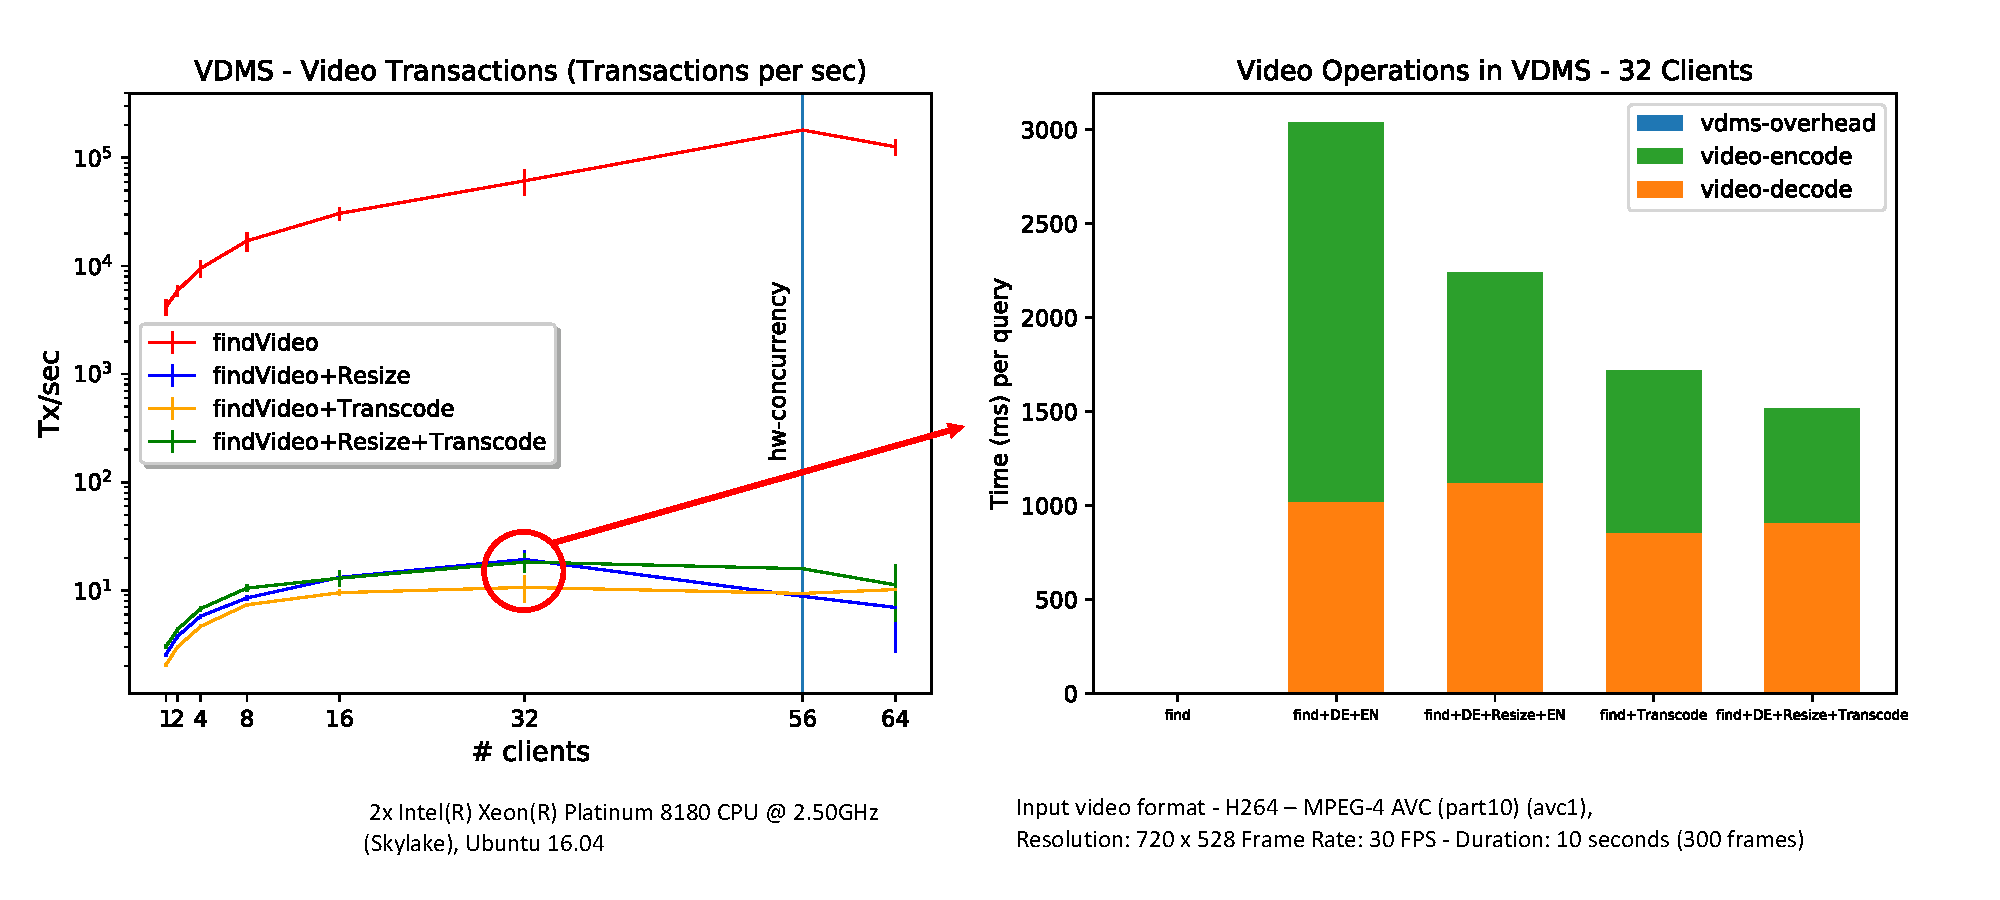
\includegraphics[width=\textwidth]{figures/video_overhead}
\caption{Analysis of video operations. The left figure shows the video throughput (videos per sec) as the number of concurrent clients increase and the right figure breaks down the different components of the
queries using 32 clients.}
\label{fig:video}
\end{figure*}

All this functionality is provided and integrated with the rest of the
metadata API as part of the comprehensive VDMS interface.
This makes it possible for users to interact with metadata and video in 
a transactional manner, enabling users to run queries like: 
"Retrieve all the videos where there is a \textit{lake} with 
probability higher than 0.86, converting all videos to \textit{H.264} 
\textit{mp4} of size 224x224".
Appendix shows a sample of how this query would be implemented using the VDMS API
\footnote{https://github.com/IntelLabs/vdms/wiki/FindVideo}.
In particular, this functionality was used internally to select a subset
of videos with the right licenses for a video summarization application.

To the best of our knowledge, there is no solution that can provide
all the functionality mentioned above, behind a single interface
that also allows users to interact with images and metadata.
Implementing a baseline, like we did for images, is significantly more complex
due to the parametrization of video encondings and containers, 
as explained at the beginning of this section.
For this reason, we chose to make a study using VDMS in various scenarios,
and analysis of scalability and the impact of having the overhead of VDMS' Request
Server in the overall access time and throughput.

Figure~\ref{fig:video} shows the analysis of different queries aimed
at retrieving a video using the VDMS interface.
We show how VDMS throughput increases when serving
a video object as the number of simultaneous clients increases, as well as the
overhead operations introduced in the overall query execution time.
The figure on the left compares the number of video transaction per second
(i.e., number of videos returned per second) when different operations
are executed as part of the transaction. The upper-bound of this would be
simply returning the video as-is (without running any encoding/decoding or
operation), represented by the red line. This query is the upper-limit because
it essentially translates to reading the video from the file-system and sending
it over a TCP/IP socket, without any other overhead or operations.

We also run a set of other queries that involve, showed in Figure~\ref{fig:video}:
(a) running a resize operation on the video and, consequently,
decoding and encoding operations as well (blue line),
(b) transcoding, meaning the use of a different container and encoder
than the one originally used (yellow line), and
(c) both resize and transcoding.
Note that the resize operation (blue and green lines) performs a downsize,
which translates in less data being sent over the wire.
This is specially noticeable when supporting 32 simultaneous clients, 
where the system provides more videos per second due to sending less data to 
the client, when compared to just transcoding and not resizing (yellow line).
We can see that the system performs best when using all the physical cores,
and this can be attributed to the compute-bound nature of video
encoding, decoding, and processing.

\begin{figure*}[ht!]
\centering
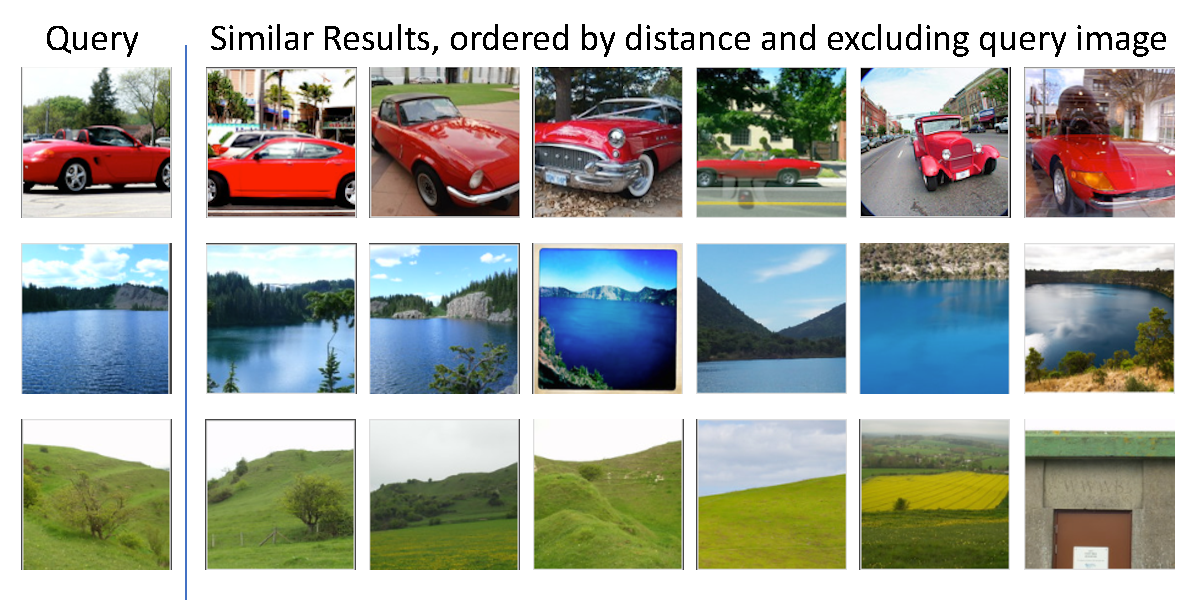
\includegraphics[width=\textwidth]{figures/feature_img_results}
\caption{Sample Results of Similarity Search}
\label{fig:similarity}
\end{figure*}

It is important to note an almost 3 orders of magnitude drop in performance
when including operations as part of the query.
We wanted to understand where most of the time was spent on the queries,
and optimize the Request Server and Visual Compute Module
if necessary. For this, we run the experiment shown at
Figure~\ref{fig:video} (right) which breaks down the different components of the
queries. This figure shows that more than 97\% of the query execution is spent
on encoding/decoding operations, which is well-known to be a
compute intensive operation\cite{videosgoogle}.
On the one hand, this result shows that VDMS barely introduces any overhead. 
On the other hand, this result means a limit on the opportunities 
for optimization for video queries given that biggest time factors 
are accounted by encoding/decoding, which is outside the scope of VDMS.
This result was the call to action for one optimization we will include
in future releases of VDMS, which involves using \textit{ffmpeg} C++ API to
limit the number of frames being encoded/decoded when possible.
This functionality will prevent encoding/decoding to happen on all frames
when users only need to retrieve a subset of the frames in the video.

%=========================================

\subsection{Similarity Search}
\label{features}

Another key differentiating factor of VDMS is that it allows the creation of
indexes for high-dimensional feature vectors and the insertion of
these feature vectors associated with entities, images, and/or videos.
Feature vectors are intermediate results of various machine
learning or computer vision algorithms when run on visual data.
Feature vectors are also known as \textit{descriptors}
or \textit{visual descriptors}. We use these terms interchangeably.
These descriptors can be classified, labeled, and used to build search
indexes. There are many in-memory libraries that are designed for
this task~\cite{flann, faiss}.
Using the VDMS API, users can manage feature vector indexes,
query previously inserted elements,
run a k-nearest neighbor search (\textit{knn}), and express relationships
between existing images or descriptors and
the newly inserted descriptors.
By natively supporting descriptors and \textit{knn},
VDMS allows out-of-the-box classification functionalities for many applications
\footnote{https://github.com/IntelLabs/vdms/wiki/ClassifyDescriptor}.

For this work, and as part of a comprehensive image search implementation,
we have used 4096-dimensional descriptors extracted from every image
(and first frame of every video) from the YFCC100M dataset
and created a collection of these feature vectors in VDMS to
perform similarity search (i.e., find images that are
\textit{similar} to an query (input) image).
\textit{Similarity} in this particular case is defined as closeness
in a 4096-dimensional space using euclidean distance as the metric.

The process of loading descriptors in VDMS is simple.
First, the user has to create a DescriptorSet, using a single command.
At creation of the DescriptorSet, the dimensionality of the descriptors
is specified, together with the desired indexing method and the desired metric
for computing distances (Euclidean Distance, \textit{L2},
or Inner Product, \textit{IP}).
Once the DescriptorSet is created, descriptors can be inserted to the set.
After the descriptors are inserted, a similarity search can be performed.

Figure~\ref{fig:similarity} shows 3 examples of a query image (on the left),
and images returned as \textit{similar} by VDMS.
The input is a descriptor generated after a query image.
The \textit{query input} descriptor is sent to VDMS as part of the query,
VDMS uses that descriptor to find similar ones,
and retrieves the images associated with those \textit{similar} descriptors.
We show this as an example of the functionality and to depict
how the feature vectors provided by the dataset can be used,
but we also provide an analytical approach to
the trade-off between accuracy and execution time in our system.
It is important to note that the accuracy of the results is entirely tied
to the quality of the descriptors chosen by the applications.
The quality of the similarity result will be tied to the quality
of the descriptor extraction that the application is using.

\begin{figure*}
\centering
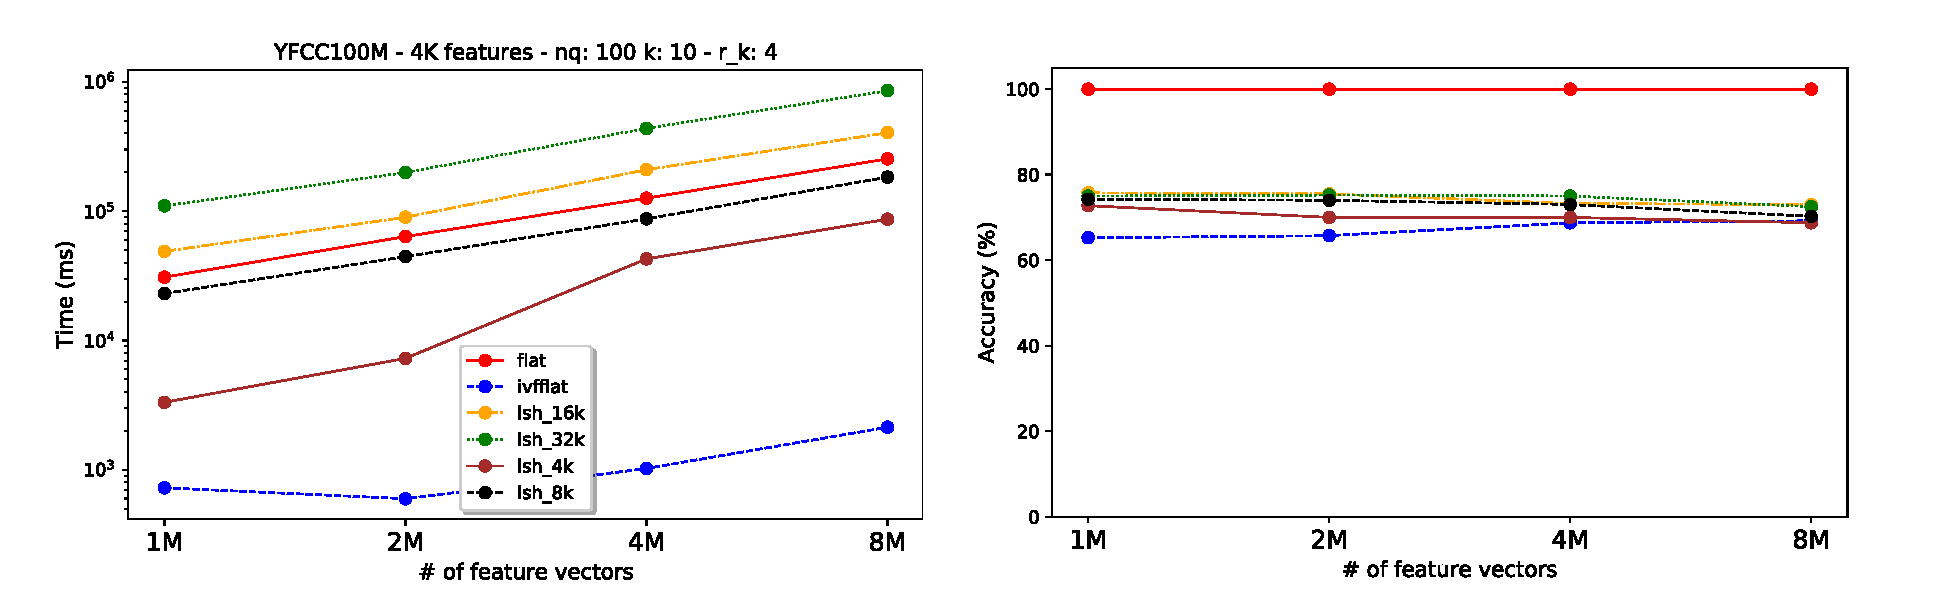
\includegraphics[width=\textwidth]{figures/features_alternatives}
\caption{Feature Vector Evaluation: Trade-off between query execution speed
and accuracy of the results, using ground-truth data for computing accuracy.
For this evaluation, we query the 10 closest neighbors (k = 10), and compute
accuracy using recall at 4 (r\_k = 4) (i.e. percentage of the top 4 ground-truth
results that is present within the top 10 computed neighbors).
We average the query execution time and accuracy for 100 queries (nq = 100).}
\label{fig:features_eval}
\end{figure*}

\begin{figure*}[ht]
\centering
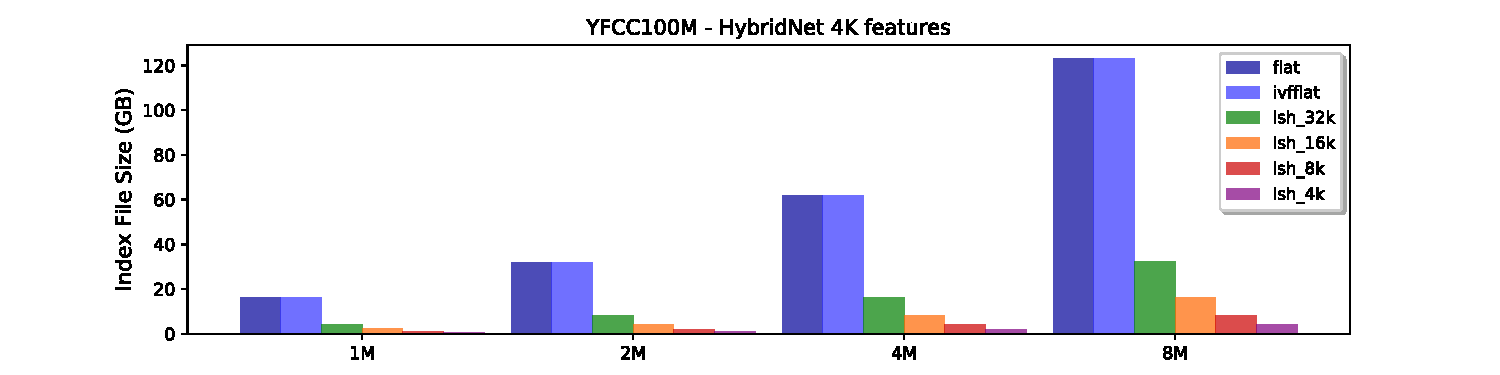
\includegraphics[width=\textwidth]{figures/features_disksize}
\caption{Feature Collection Size in Disk}
\label{fig:features_size_does_matter}
\end{figure*}

As mentioned before, VDMS provides different levels of customization of the
indexes created for a descriptor set, that includes the indexing techniques
and the metric for similarity.
These different indexing techniques come with different trade-offs in terms
of speed of search and accuracy of the computation.
VDMS aims to provide functionality that is agnostics to application-specific
techniques, enabling features that are generic to visual data processing
applications.
Figure~\ref{fig:features_eval} shows an analysis at the different indexing
techniques provided by VDMS and its trades-off between accuracy and query
execution speed, for a single threaded client.
For this evaluation, we query the 10 closest neighbors (k = 10), and compute
accuracy using recall at 4 (r\_k = 4) (i.e. percentage of the top 4 ground-truth
results that is present within the top 10 computed neighbors).
We average the query execution time and accuracy for 100 queries (nq = 100).
The \textit{flat} index (red line) implements exact search and
represents ground-truth, which explain why the
accuracy is always 100\% in the plot on the right.
The other indexes implement \textit{approximate search},
which trades-off between accuracy and speed of search~\cite{flann, faiss}.
We have also tried the \textit{ivfflat} index (inverted file index), as well as
\textit{LSH}-based indexes using a different number of bits per descriptor
\footnote{https://github.com/facebookresearch/faiss/wiki/Faiss-indexes}.
Results show how \textit{ivfflat} is the fastest option but it comes with a trade-off
of about 30\% loss in accuracy, while simple brute-force search
is among the slowest options at the expenses of 100\% accuracy,
meaning exact search.

Another important trade-off to be made is with respect to space efficiency:
The DescriptorSet can grow very large and expensive to load and manage.
In this particular case, 4096-dimensional descriptors for 100M elements
translates into 1TB of data, only in raw floating-point data alone
(without accounting for any metadata or indexes associated with it).
This component is very important for the overall analysis on which
index structure to use because a large set of descriptors may not fit in memory
and thus cause a pressure on the IO system while retrieving descriptors
for computing distance.
This can severely impact the overall query execution time.
When the DescriptorSet grows significantly large,
it may be worth trading off accuracy for speed and space.
Figure~\ref{fig:features_size_does_matter} shows the different indexes and
their size in disk. These indexes already contain all the descriptors (or
a quantized version of them in the case of LSH~\cite{lsh}),
and can be loaded in memory directly when it fits.
Note how, because of quantization of the descriptors, \textit{LSH} provides a
significantly lower space foot print, which can be a great option for
large collections of descriptors when accuracy is not a main factor.
It is not uncommon to sacrifice accuracy as images and videos are captured
using a noise sensor (i.e., the camera), and an approximate search
in many cases can provide the necessary accuracy for applications
to achieve their goals.
